\documentclass[tikz, border = 10pt]{standalone}
\renewcommand{\familydefault}{\sfdefault} 

\usetikzlibrary{positioning, quotes, calc, arrows.meta, bending, shapes, backgrounds}

\tikzset{
every node/.style = {scale = 1.1},
manifest/.style = {rectangle, draw, thin, inner sep = 5pt, minimum width = 1cm, 
	minimum height = 1cm},
latent/.style = {ellipse, draw, thin, inner sep = 5pt, minimum width = 1cm, 
	minimum height = 1cm},
residual1/.style = {circle, draw, thin, minimum size = 5mm, inner sep = 1pt}, 
residual2/.style = {rectangle, minimum width = 0.5pt, minimum height = 1.5mm, 
	inner sep = 0pt, outer sep = 0mm},
regression/.style = {-{Stealth[length = 1.5mm]}, thin, shorten > = 1pt, inner sep = 2pt},
covariance/.style={{Stealth[length = 1.5mm]}-{Stealth[length = 1.5mm]}, thin, 
	shorten > = 1pt, shorten < = 1pt, inner sep = 2pt},
variance/.style={{Stealth[length = 1mm]}-{Stealth[length = 1mm]}, thin, 
	shorten > = 1pt, shorten < = 1pt, inner sep = 1.5pt},
interaction/.style = {-{Stealth[sep = 1pt, length = 1.5mm] . Circle[length = 4pt]}, 
	thin, shorten > = -2pt},
constant/.style = {draw, thin, inner sep = 1pt, regular polygon, 
    regular polygon sides = 3, minimum size = 5mm}
}

\begin{document}
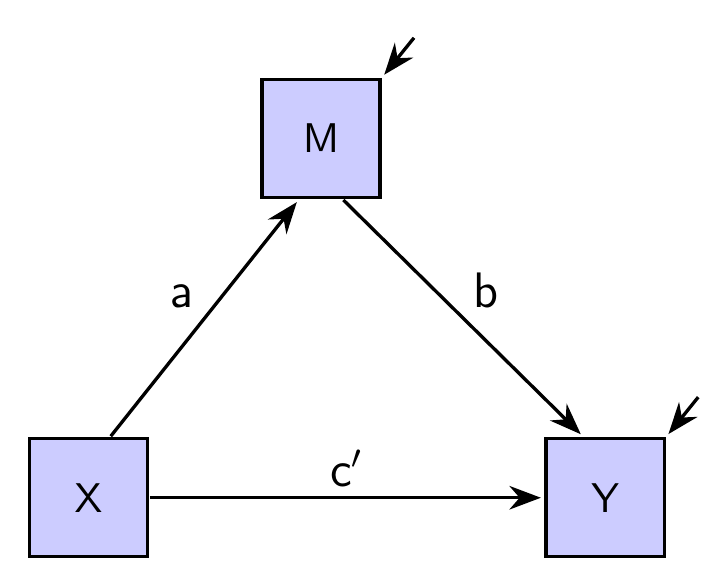
\begin{tikzpicture}
\tikzset{every node/.style = {scale = 1.5},
regression/.style = {-{Stealth[length = 4mm]}, very thick, shorten > = 1pt, inner sep = 2pt}}

%% The manifest variables
\node [manifest, very thick, fill = blue!20] (X) {X};
\node [manifest, very thick, fill = blue!20] (Y) [right = 5cm of X] {Y};
\node [manifest, very thick, fill = blue!20] (M) [above = 3cm of $(X.north) !0.45! (Y.north)$] {M};

%% The regressions
\path [regression] (X) edge ["\large{c$'$}"] (Y);
\path [regression] (X.70) edge ["\large{a}"] (M.250);
\path [regression] (M.290) edge ["\large{b}"] (Y.110);

%% The residuals and their variances
\node [residual2] (e2) [above right = 4mm and 4mm of Y] {};
\node [residual2] (e1) [above right = 4mm and 4mm of M] {};
\path [regression] (e2) edge (Y.north east);
\path [regression] (e1) edge (M.north east);

\end{tikzpicture}
\end{document}
